% !TeX program = pdflatex
\documentclass[12pt,a4paper]{article}

% Essential packages
\usepackage[utf8]{inputenc}
\usepackage[T1]{fontenc}
\usepackage[polish]{babel}
\usepackage{csquotes}
\usepackage{amsmath}
\usepackage{hyperref}
\usepackage{xcolor}
\usepackage{geometry}
\usepackage{booktabs}
\usepackage{float}  
\usepackage{array}    
\usepackage[backend=biber,style=numeric,sorting=none]{biblatex}
\usepackage{graphicx}
\usepackage{tocloft}  % For customizing table of contents
\usepackage{enumitem} % For better list formatting
\usepackage{listings} % For code listings with line wrapping

\geometry{
    a4paper,
    margin=2.5cm
}

% Listings package configuration
\lstset{
  basicstyle=\ttfamily\small,
  breakatwhitespace=false,
  breaklines=true,
  postbreak=\mbox{\textcolor{red}{$\hookrightarrow$}\space},
  showstringspaces=false
}


% Table of contents settings
\renewcommand{\cftsecleader}{\cftdotfill{\cftdotsep}}
\renewcommand{\cftsubsecleader}{\cftdotfill{\cftdotsep}}
\setcounter{tocdepth}{2}  % Show sections and subsections in TOC
\setcounter{secnumdepth}{2}  % Number sections and subsections

% Hyperref settings
\hypersetup{
    colorlinks=true,
    linkcolor=blue,
    filecolor=magenta,
    urlcolor=cyan,
    pdftitle={Raport końcowy: Równoległy System Analizy Roślinności Sentinel-2},
    pdfauthor={Adrian Rybaczuk, Bartosz Cylwik},
    pdfsubject={Przetwarzanie Rozproszone i Równoległe},
    pdfkeywords={Sentinel-2, NDVI, NDMI, Przetwarzanie Równoległe, Python, GUI}
}


\title{Projekt zaliczeniowy\\\large Raport końcowy}
\author{Zespół Projektowy nr 1 \\
    \begin{tabular}{ll}
        \textbf{Adrian Rybaczuk} & \textbf{318483} \\
        \textbf{Bartek Cylwik} & \textbf{325457} \\
    \end{tabular}
}
\date{\today}


% Bibliography file
\addbibresource{references.bib}
\selectlanguage{polish} % Set language to Polish
\begin{document}

\maketitle

\begin{abstract}
Treść z isoda - temat 2:\\
Implementacja (wraz z GUI) równoległego / rozproszonego mechanizmu wyliczania indeksów wilgotności (NDMI) i wegetacji (NDVI) roślin na zobrazowaniach satelitarnych (produktach z systemu Copernicus; Sentinel-2) do stwierdzania występowania lub zaniku roślinności (ich kondycji) na wskazanym obszarze.
\end{abstract}
  

\tableofcontents
\newpage


\section{Wprowadzenie}
Celem projektu była implementacja systemu równoległego lub rozproszonego mechanizmu wyliczenia indeksów NDMI i NDVI, czyli wiglotnosći i wilgotności na świecie. Dane jak mówi treść zadania pozyskaliśmy z zobrazowań satelitarnych Sentinel-2.
Stworznie porjektu, rozdzieliliśmy na poniższe aspekty:
\begin{itemize}
    \item Wybranie technologi do realizacji projektu \ Zdecydowaliśmy na pythona, gdyż sprawdziliśmy, że ma bibloteke do sentinela, no i inne przydatne w wyodrębnianiu/ rekonstrukcji danych.
    
    \item Uzyskanie wskaźników NDVI i NDMI
    \begin{itemize}
        \item Wzory oraz wiedza ogólna jak są wykorzystywane
        \item Pobranie niezbędnych wskaźników z zobrazowania satelitarnego Sentinel-2
        \item Zapisanie danych pobranych z API w cashu, żeby uniknąć ponownego pobierania danych
        \item Identyfikacja potęcjalnych problemów związanych z przetwarzaniem danych
        \item Przeprowadzenie obliczeń wskaźników przy sekcji równolełej programu
    \end{itemize}
    \item Interfejs graficzny
    \begin{itemize}
        \item Uwierzytelniania z API Sentinelhuba
        \item Głowny ekran, w którym możemy wybrac jako parametry okres danych do pobrania, zakres współrzednych jak i sposób wyliczenia współczynników.
        Rónież i tu pojawią sie obok obszaru dane pokrycie na mapie współczynnikami dla wybranych pikseli obrazu
        \item Sekcja wyników, gdzie przeprowadzamy na zgromadzonych danych testy wydajnościowe, w celu porównania obliczeń między cpu a gpu, oraz wpływ ilości wątków.
    \end{itemize}
    \item Równoległe przetwarzanie
    \begin{itemize}
        \item Zastosowanie równoleóosci jedynie w obrębie samego liczenia współćzynników, są to tysiące-miliony danych, a GPU jest wydajny gównie w takich przypadkach.
        \item Wspomniany wybór pomiedzy przetwarzaniem na CPU a GPU
    \end{itemize}
\end{itemize}

\newpage

\section{Kroki podjęte na początku pracy}

\subsection{Następnym krokiem będzie uzyskanie dostępu do danych z Sentinel-2}

Do tego celu skorzystaliśmy z API Sentinel-Hub. \cite{sentinel2_api_docs} 
Udostępnia on dane z satelity poprzez API dopiero po uwierzytelnieniu. 
W tym celu musielismy przejść przez process opisany w tym odnośniku \cite{sentinel2_api_docs_auth}.
Po jego przejsciu mamy dostep do Client ID oraz Client Secret które wykorzystamy do połączenia się z API.

API posiada reate limiting. 
\cite{sentinel2_api_auth_rate_limiting}
Z tego też powodu zamierzamy wykorzystać cache do przechowywania pobranych już danych.
Z natury projektu i dania sobie możliwości testowania wyników zamierzamy przechowywać nieprzetworzone dane zamiast obliczonych już wyników.
Pomoże nam to przeprowadzić testy i wprowadzić poprawki w przyszłości.

\subsection{Research wskaźników NDVI i NDMI}

\textbf{NDVI} (Normalized Difference Vegetation Index) \cite{ndvi_docs} jest prostym wskaźnikiem ilościowym. Służy on do klasyfikacji wegetacji roślin. Jego wartość mieści się w przedziale od $-1$ do $1$: czyli od mocnego występowania wody do bujnej flory

Wzór NDVI :
\[
\mathrm{NDVI} = \mathrm{Index}(\mathrm{NIR}, \mathrm{RED}) = \frac{\mathrm{NIR} - \mathrm{RED}}{\mathrm{NIR} + \mathrm{RED}}
\]

W przypadku danych Sentinel-2, indeks ten wyznaczamy na podstawie kanałów B8 (NIR) i B4 (RED):
\[
\mathrm{NDVI} = \mathrm{Index}(\mathrm{B8}, \mathrm{B4}) = \frac{\mathrm{B8} - \mathrm{B4}}{\mathrm{B8} + \mathrm{B4}}
\]

\textbf{NDMI} (Normalized Difference Moisture Index) \cite{ndmi_docs} -znormalizowany wskaźnik wilgotności, który do wyznaczenia wilgotności wykorzystuje pasma NIR i SWIR.
W tym samym przedziale co NDVI, wskazuje od suchych obszarów do mocno wilgotnych.

Wskaźnik NDMI definiujemy wzorem:
\[
\mathrm{NDMI} = \mathrm{Index}(\mathrm{NIR}, \mathrm{SWIR}) = \frac{\mathrm{NIR} - \mathrm{SWIR}}{\mathrm{NIR} + \mathrm{SWIR}}
\]

W przypadku danych Sentinel-2, indeks ten wyznaczamy na podstawie kanałów B8 (NIR) i B11 (SWIR):
\[
\mathrm{NDMI} = \mathrm{Index}(\mathrm{B8}, \mathrm{B11}) = \frac{\mathrm{B8} - \mathrm{B11}}{\mathrm{B8} + \mathrm{B11}}
\]

\subsection{RED, NIR, SWIR czyli B4, B8, B11}

\textbf{RED} czerwony kanał światła, silnie odbijany przez martwe liście. Wykorzystywany do identyfikacji typów roślinności, gleb, obszarów zabudowanych itd.

Dla Sentinel-2 to B4: \cite{sentinel2_band_B4}
\begin{itemize}
    \item Rozdzielczość: 10 m/px
    \item Centralna długość fali: 665 nm
    \item Szerokość pasma: 30 nm
\end{itemize}

\textbf{NIR} (Near Infrared) to bliska podczerwień, która dobrze obrazuje linie brzegowe oraz zawartość biomasy.

W Sentinel-2 kanał NIR odpowiada pasmu B8: \cite{sentinel2_band_B8}
\begin{itemize}
    \item Rozdzielczość: 10 m/px
    \item Centralna długość fali: 842 nm
    \item Szerokość pasma: 115 nm
\end{itemize}

\textbf{SWIR} (Short-Wave Infrared) jest to fala wysokowrażliwa na zawartość wody w obiektach. Dlatego jest dobrym wskaźnikiem wilgotności.

W Sentinel-2 kanał SWIR odpowiada pasmu B11: \cite{sentinel2_band_B11}
\begin{itemize}
    \item Rozdzielczość: 20 m/px
    \item Centralna długość fali: 1610 nm
    \item Szerokość pasma: 130 nm
\end{itemize}

Poczatkowo zakladalismy koniecznosc recznego przeskalowania pasm Sentinel-2 o roznych rozdzielczościach, aby je ujednolicić. Jednak API Sentinel Hub automatycznie dostarcza je w najwyzszej wspolnej rozdzielczosci (10 m/px), co uproscilo przetwarzanie danych.

\subsection{Zrównoleglenie / rozproszenie obliczeń}
W związku z tym, że chcieliśmy, by aplikacja działała na jednym komputerze, wybraliśmy ścieżkę zrównoleglenia obliczeń. Zadanie obliczania wskaźników polega na wykonaniu prostych operacji arytmetycznych dla milionów pikseli.

Zakładaliśmy, że obliczenia na GPU, ze względu na ich masowo równoległą architekturę, będą najwydajniejszym rozwiązaniem. Aby się o tym przekonać, dodajemy do naszej aplikacji testy, przedstawiające w outpucie analizę związaną z różnymi strategiani obliczeniowymi:
\begin{enumerate}
    \item \textbf{Przetwarzanie na GPU} z wykorzystaniem języka Taichi, aby zbadać potencjał masowego zrównoleglenia.
    \item \textbf{Równoległe przetwarzanie na CPU} z wykorzystaniem modułu \texttt{multiprocessing} i pamięci dzielonej, aby ocenić skalowalność na wielordzeniowych procesorach.
    \item \textbf{Jednowątkowe przetwarzanie na CPU} z wykorzystaniem wysoce zoptymalizowanej biblioteki NumPy, służące jako nasz główny punkt odniesienia.
\end{enumerate}

\subsection{Wybór technologii}

Jako że określiliśmy już dokładniej ramy projektu możemy potwierdzić wybrane przez nas technologie. 
Ogólny język implementacji to Python.
Do pobierania danych z api wykorzystaliśmy bibliotekę SentinelHub. Która udosptępnia już gotowe funkcje pozwalające zautoryzować się z api oraz pobrać dane.
Do gui wykorzystaliśmy Tkinter podstawową i dosyć prostą bibliotekę do tworzenia interfejsu graficznego.
Do prezentacji mapy wykorzystaliśmy TkinterMapView.
Do zrównoleglenia obliczeń skorzystamy z Taichi Lang \cite{taichi_lang_docs} którego zaembedujemy w pythonie.
Jest to język programowania osadzony w pythonnie stworzony do wysokowydajnych obliczeń.
Jego zaletą jest to że kod napisany raz przekąpiluje się na wiele różnych platform.

\newpage

\section{Przebieg procesu w aplikacji}
Aplikacja została zaprojektowana z myślą o prostocie i intuicyjności obsługi. Interakcja użytkownika z systemem przebiega w kilku logicznych krokach:
\begin{enumerate}
    \item \textbf{Uwierzytelnianie:} CliendId i ClientSecret oraz własne hasło. Przy nastepnym logowaniu wystarczy hasło.
    \item \textbf{Główny widok mapy:} Po pomyślnym zalogowaniu, użytkownik przechodzi do głównego interfejsu, który składa się z dwóch głównych paneli: interaktywnej mapy satelitarnej na któej może wybrać współrzędne oraz pole na okres pobieranych danych. Z boku jest panel na wyniki obliczeń indeksów.
    \item \textbf{Wybór sposobu liczenia:} ] W górnym panelu dostępne są kontrolki do wyboru zakresu dat oraz metody przetwarzania (GPU lub CPU).
    \item \textbf{Pobieranie danych:} Jest przycisk "Fetch Data" gdzie aplikacja wysyła zapytanie do API Sentinel Hub o pasma B4, B8, B11 oraz maskę danych dla widocznego na ekranie obszaru. Pobrane dane są zapisywane w lokalnym folderze 
    \item \textbf{Obliczenia i wizualizacja:} Po pobraniu danych, aktywują się przyciski "Calculate NDVI" i "Calculate NDMI". Kliknięcie jednego z nich uruchamia obliczenia w osobnym wątku (aby nie blokować interfejsu), wykorzystując wybraną metodę. Po zakończeniu obliczeń, z prawje strony wyświetlana jest heatmapa wskaźnika wraz z legendą.
    \item \textbf{Moduł testowy:} Z widoku mapy można przejść do dedykowanego panelu testowego, który pozwala na uruchomienie serii testów wydajnościowych i wygenerowanie  wykresów porównujących zaimplementowane metody obliczeniowe.
\end{enumerate}

\section{Równoległe przetwarzanie}

\subsection{Które obliczenia i dlaczego postanowiliśmy zrównoleglić}
Głównym kandydatem do zrównoleglenia w naszym projekcie były obliczenia wskaźników NDVI i NDMI. Decyzja ta wynikała z charakterystyki problemu:
\begin{itemize}
    \item \textbf{Niezależność danych (Data Parallelism):} Wartość wskaźnika dla każdego piksela obrazu satelitarnego jest obliczana wyłącznie na podstawie wartości pasm dla tego samego piksela. Nie ma żadnych zależności między sąsiednimi pikselami.
    \item \textbf{Duża skala problemu:} Obrazy satelitarne mogą składać się z milionów lub więcej pikseli. Wykonywanie operacji na tak dużej liczbie danych w sposób sekwencyjny się mija z celem.
    \item \textbf{Powtarzalność operacji:} Ten sam, prosty wzór matematyczny \((a-b)/(a+b)\) jest stosowany dla każdego piksela.
\end{itemize}

\subsection{Jak dokonaliśmy zrównoleglenia obliczeń}
Aby przeprowadzić kompleksową analizę, zaimplementowaliśmy trzy różne strategie obliczeniowe:

\subsubsection{Przetwarzanie na GPU z użyciem Taichi Lang}
Wykorzystaliśmy Taichi jako kompilator JIT do równoległego przetwarzania danych na GPU, co pozwoliło nam błyskawicznie wykonywać obliczenia \(\frac{a-b}{a+b}\) na tysiącach pikseli jednocześnie.

\subsubsection{Równoległe przetwarzanie na CPU z użyciem `multiprocessing`}
Tutaj dzięki mechanizmowi pamięci dzielonej mogliśmy równolegle przetwarzać dane na wielu rdzeniach CPU bez kosztownego kopiowania.

\subsubsection{Jednowątkowe przetwarzanie na CPU z użyciem NumPy}
Stworzyliśmy także szybki, jednowątkowy baseline w NumPy, korzystający z natywnych, zoptymalizowanych funkcji w C i Fortranie.

\section{Platforma Testowa}
Testy wydajnościowe zostały przeprowadzone na jednolitej platformie sprzętowej dostepny widok z głownego dashbordu naszej aplikacji. Poniższa specyfikacja dokumentuje konfigurację komputera użytego do testów. 

\begin{description}
    \item[System Operacyjny:] Windows 10 (AMD64)
    \item[Procesor (CPU):] AMD Ryzen 9 3900X
    \item[Szczegóły CPU:] 12 rdzeni fizycznych / 24 wątki, Taktowanie bazowe: 3.8 GHz, Cache L2: 6 MB, Cache L3: 64 MB
    \item[Pamięć RAM:] 64 GB DDR4
    \item[Karta Graficzna (GPU):] AMD Radeon RX 6800 XT
\end{description}

\textit{Uwaga: Na wydajność, zwłaszcza w przypadku obliczeń na GPU, mają również wpływ czynniki nieujęte w powyższej specyfikacji, takie jak wersja i przepustowość magistrali PCIe, szybkość pamięci VRAM oraz ogólne obciążenie systemu podczas testów.}

\section{Jakie wyniki uzyskaliśmy}
W celu oceny wydajności zaimplementowanych metod, przeprowadziliśmy serię testów,
które polegały na mierzeniu czasu wykonania obliczeń dla danych o różnej rozdzielczości oraz analizie zużycia pamięci. Oto otrzymane wykresy:

\begin{figure}[H]
    \centering
    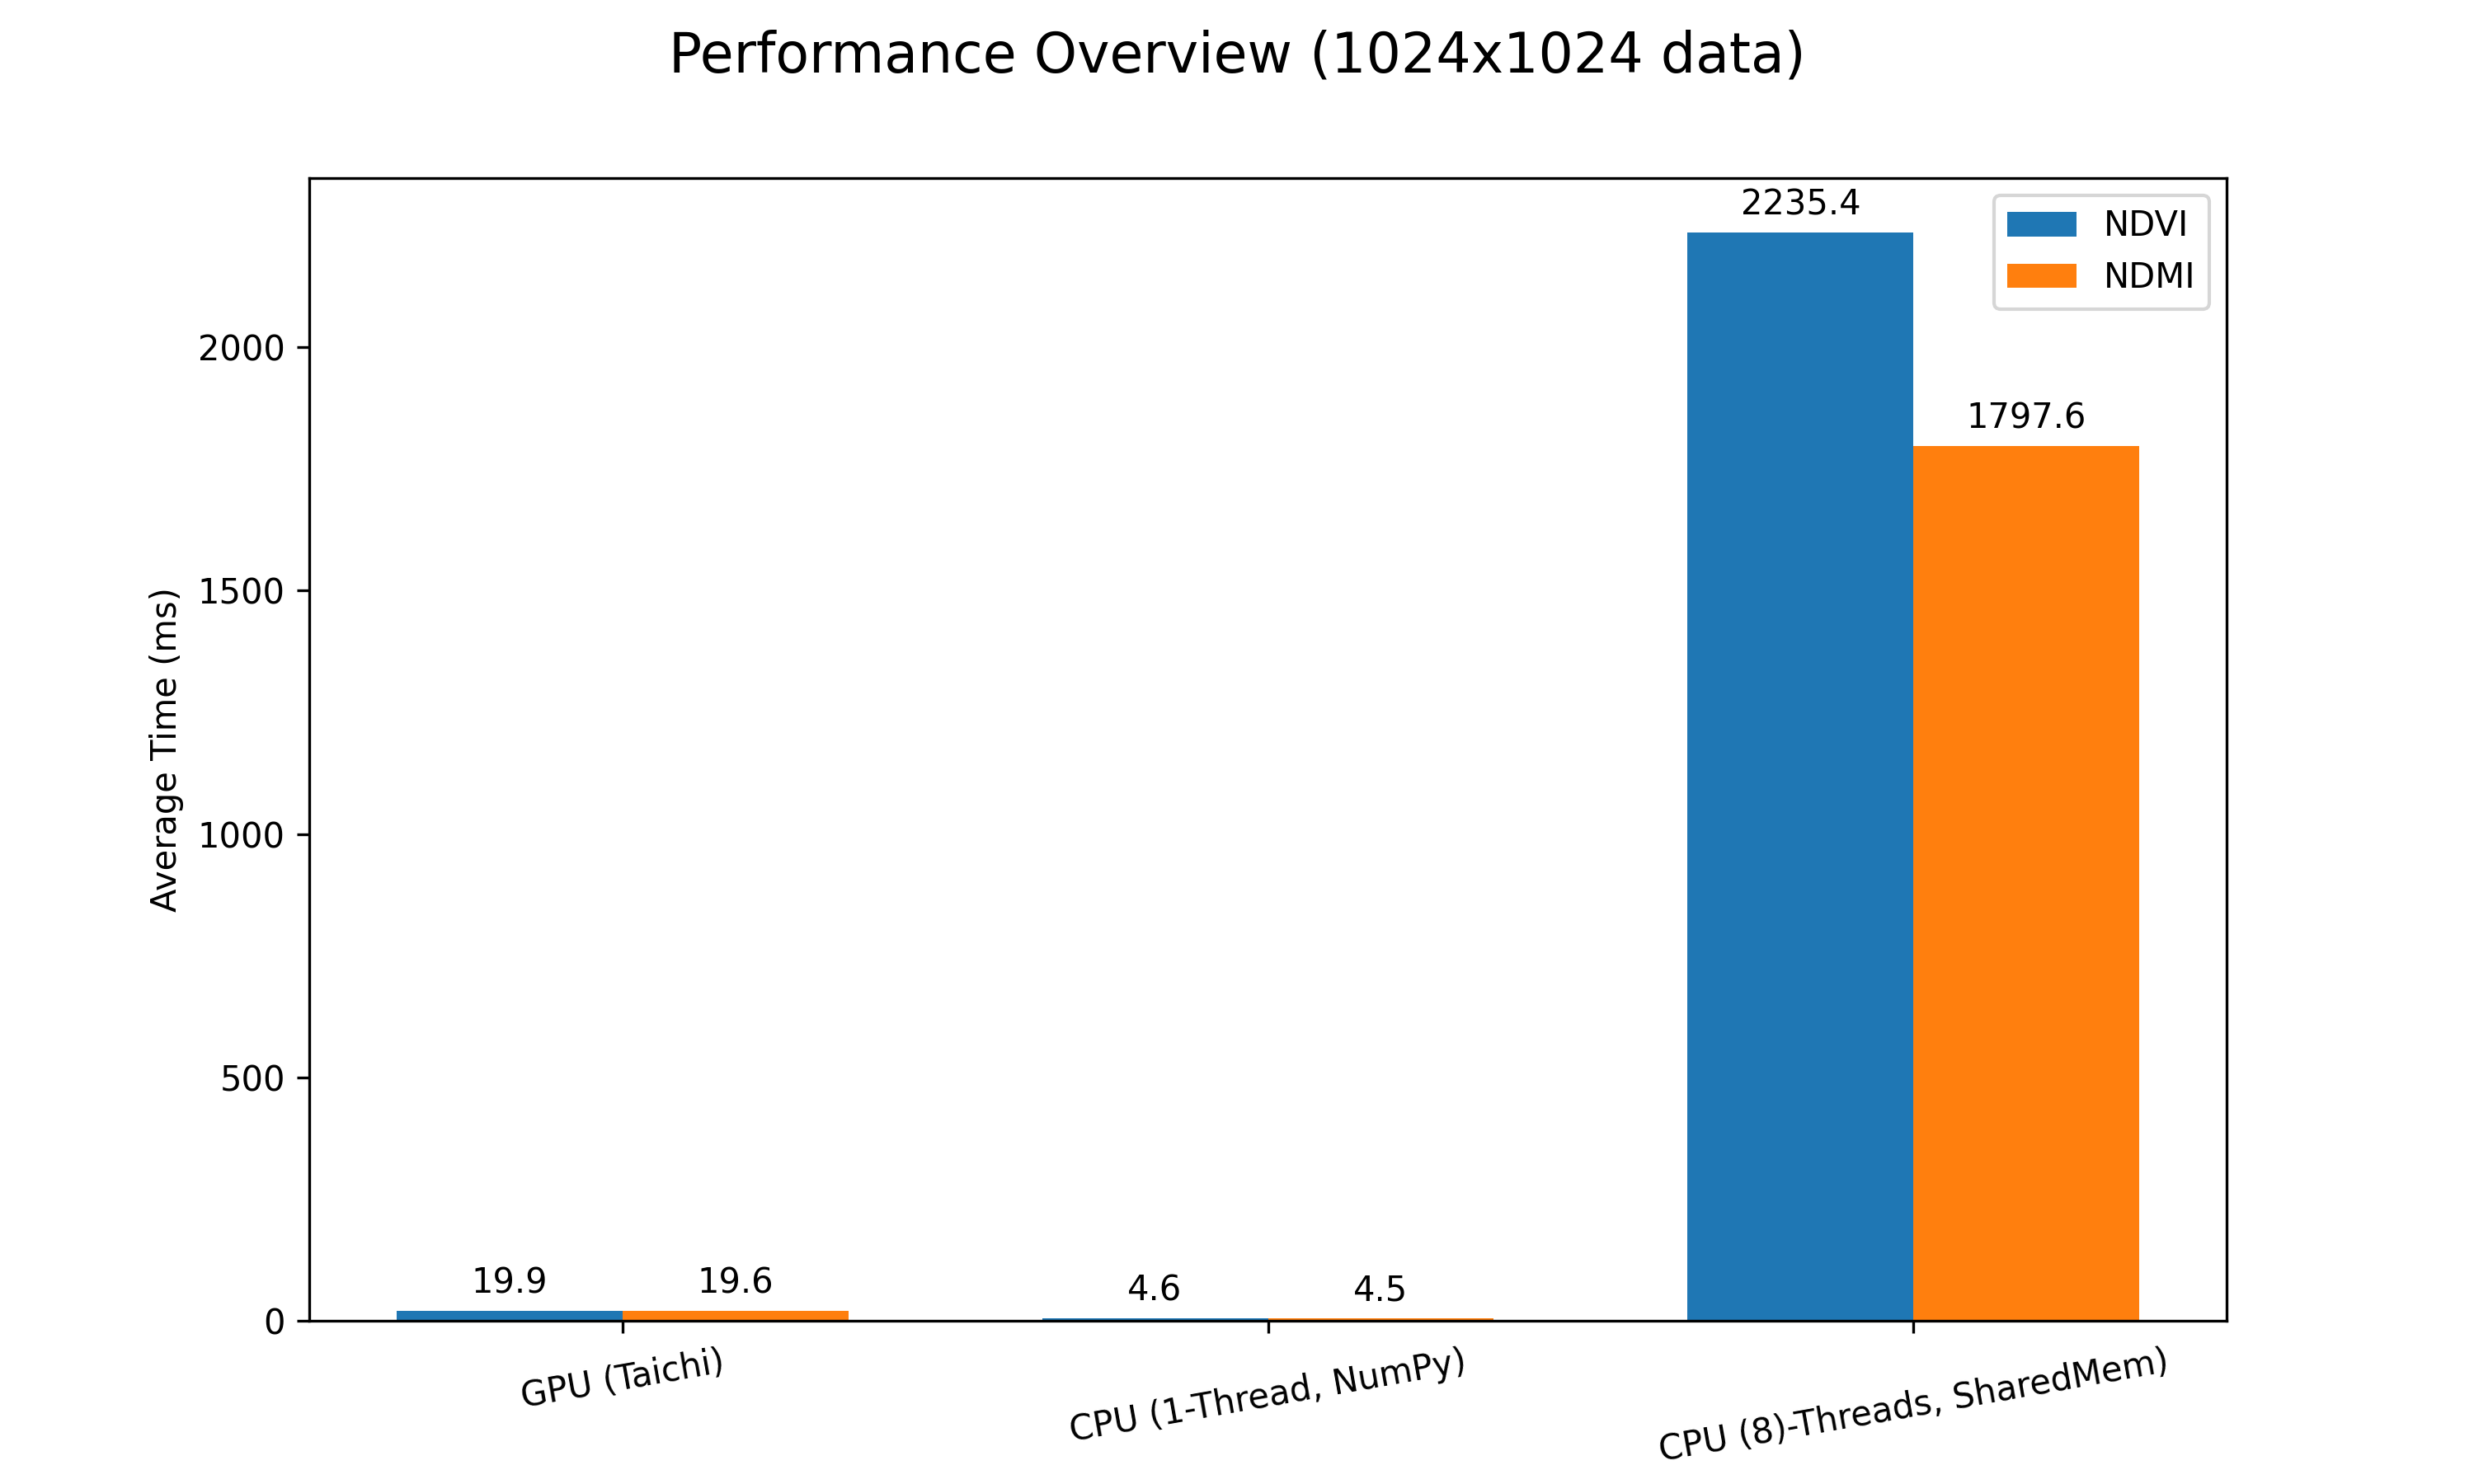
\includegraphics[width=0.8\textwidth]{charts/01_performance_overview.png}
    \caption{Przegląd wydajności dla danych 1024x1024.}
    \label{fig:overview}
\end{figure}

\begin{figure}[H]
    \centering
    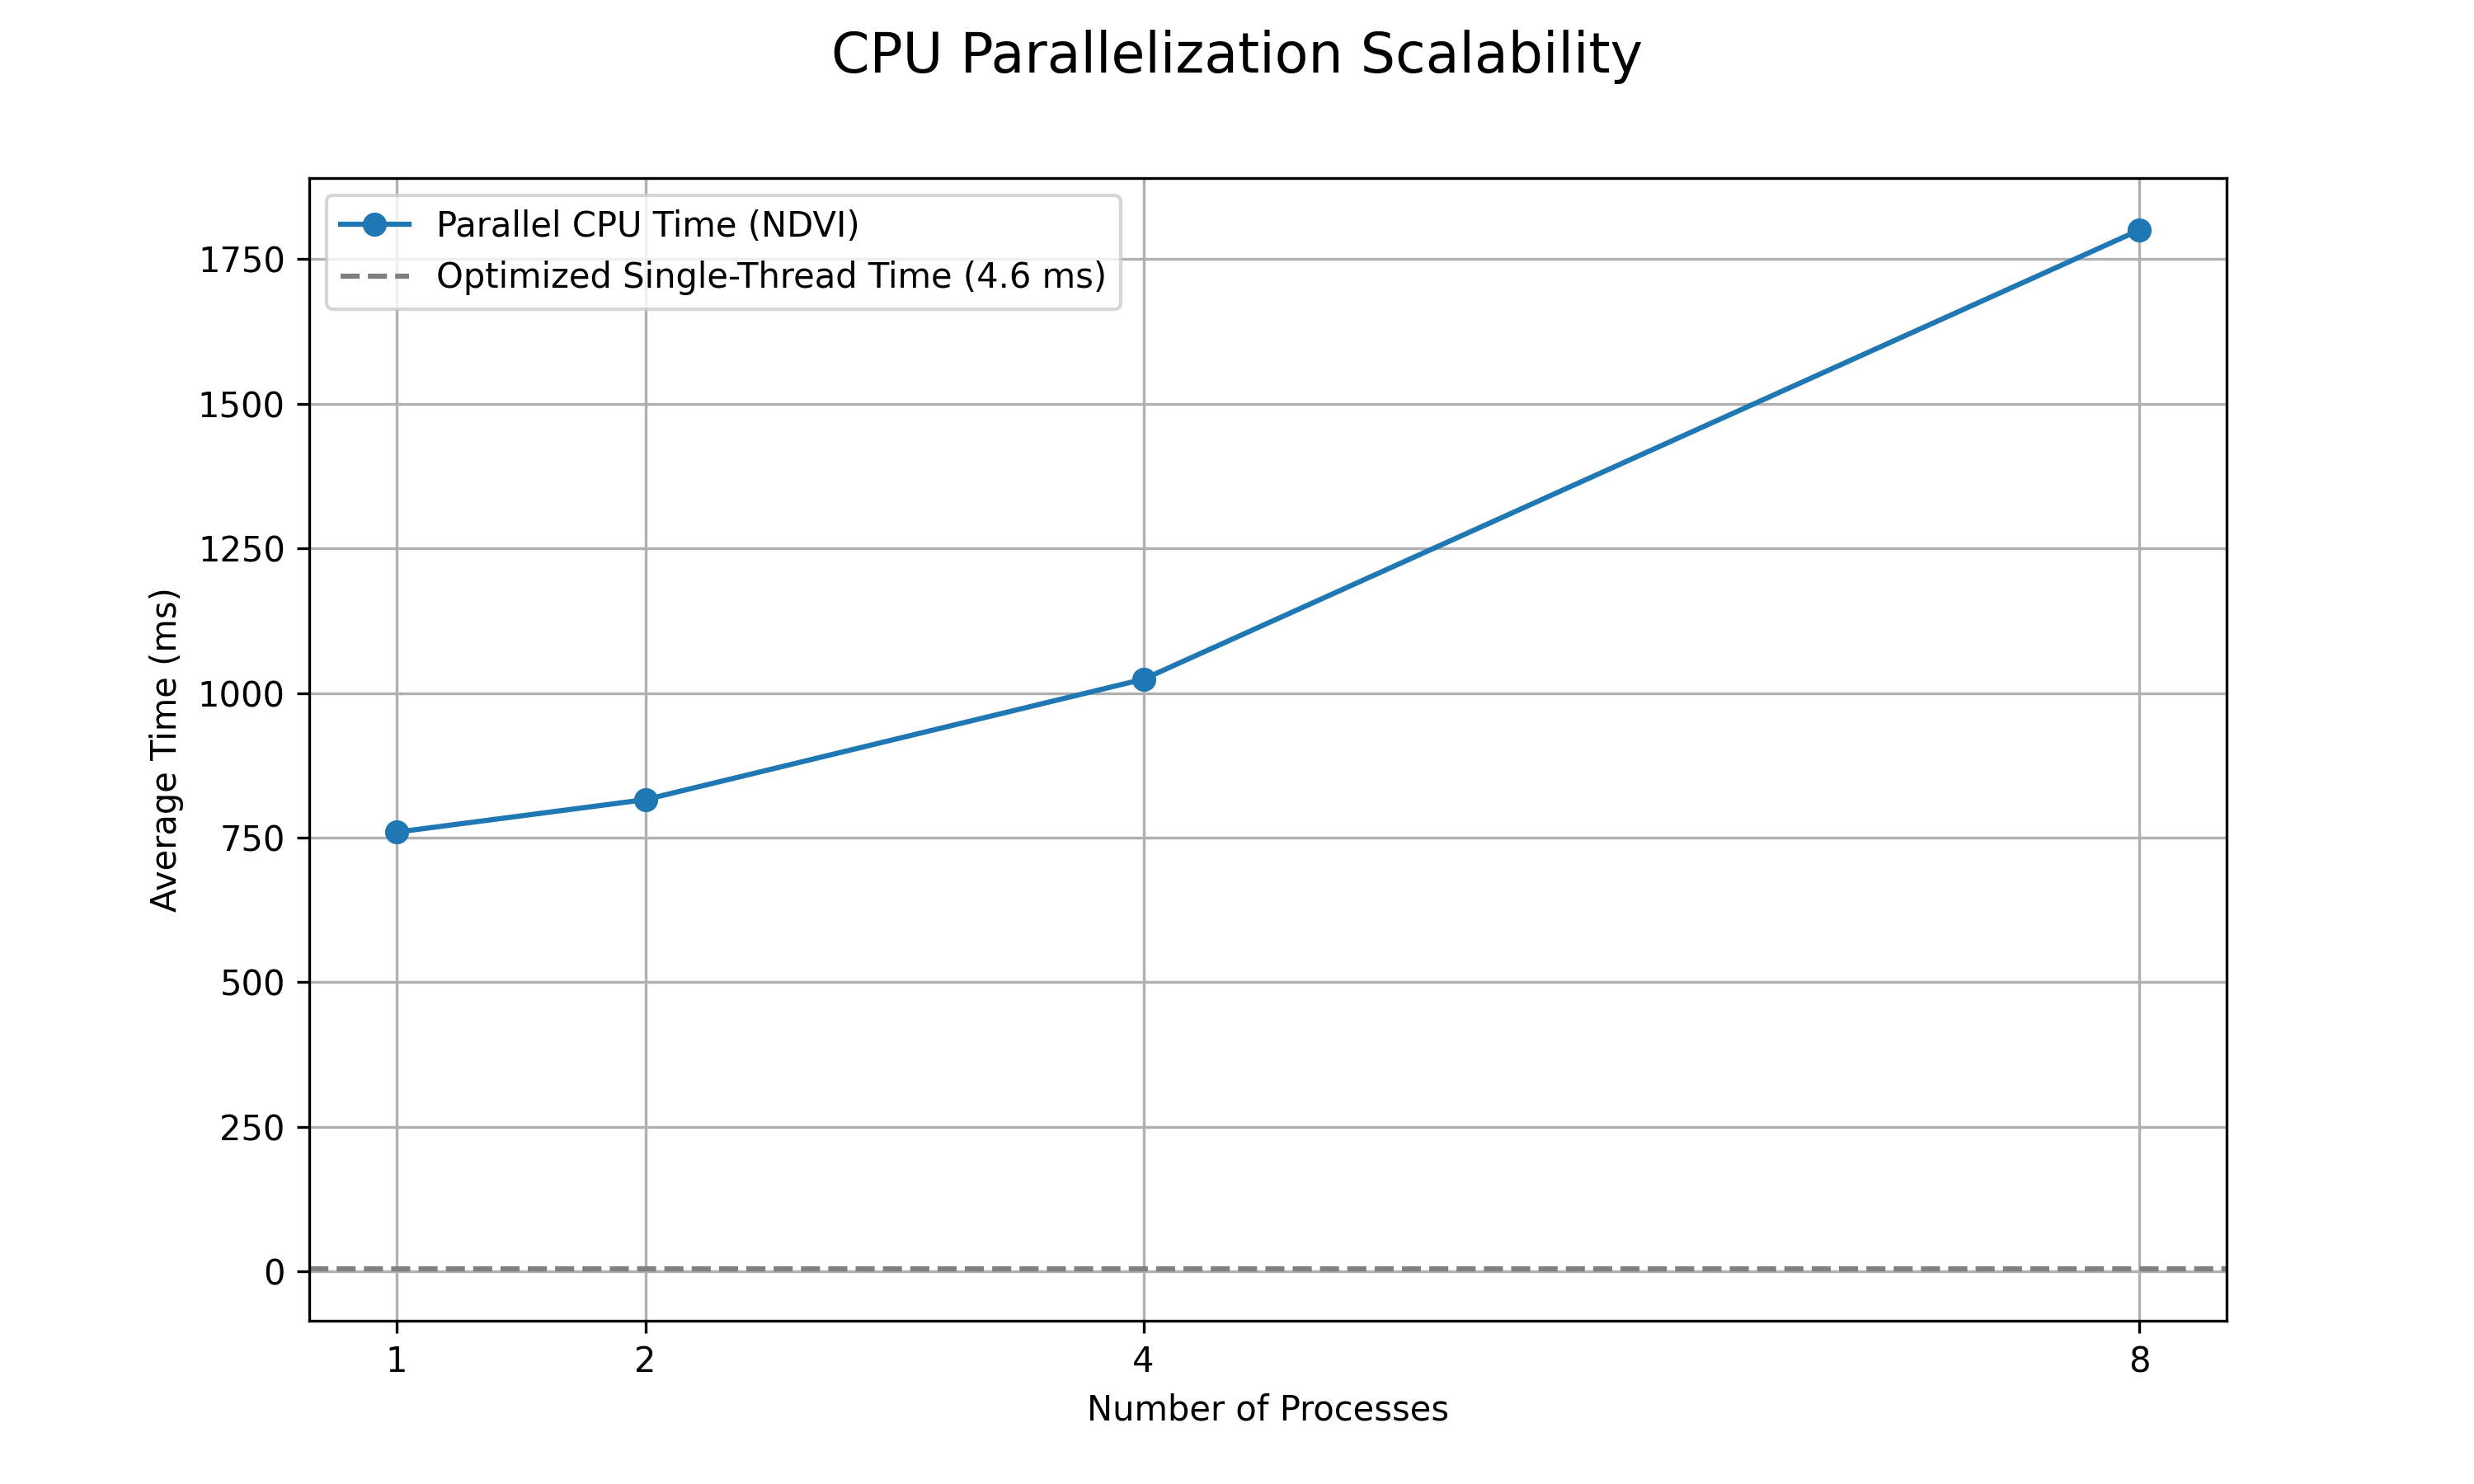
\includegraphics[width=0.8\textwidth]{charts/02_cpu_scalability.png}
    \caption{Analiza skalowalności implementacji równoległej na CPU.}
    \label{fig:cpu_scaling}
\end{figure}

\begin{figure}[H]
    \centering
    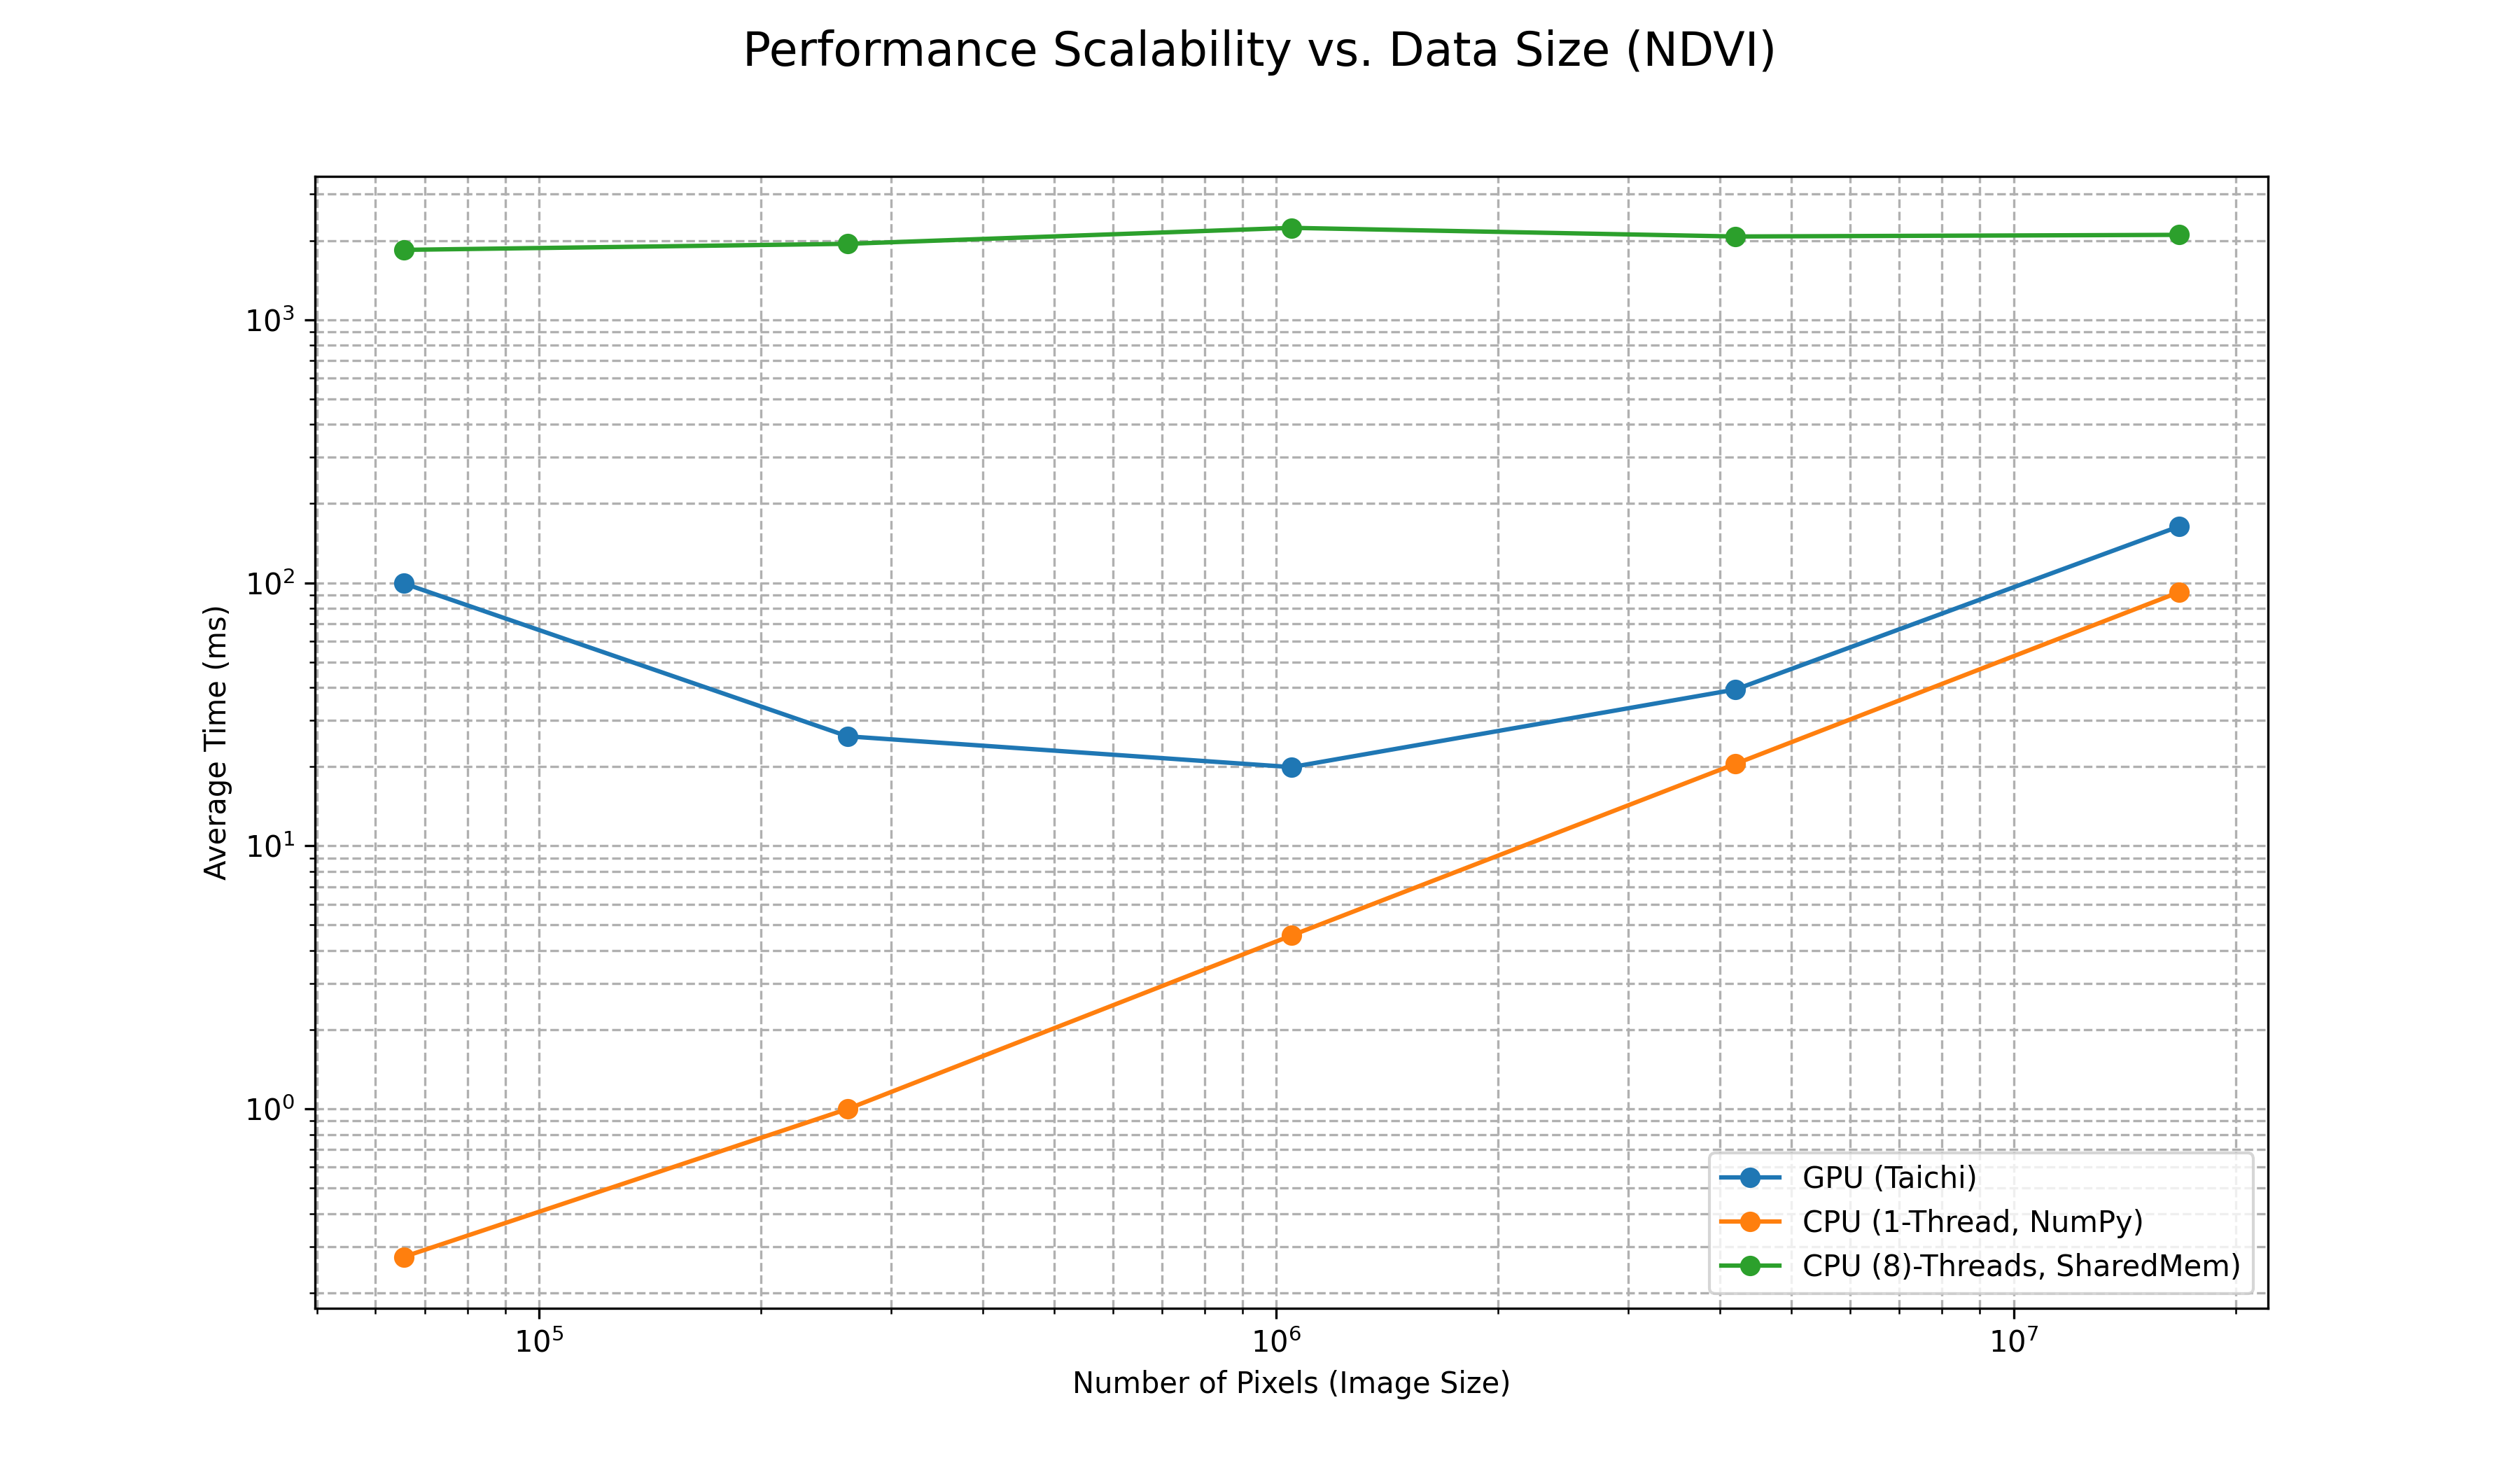
\includegraphics[width=\textwidth]{charts/03_size_scalability_ndvi.png}
    \caption{Skalowalność wydajności w zależności od rozmiaru danych (NDVI).}
    \label{fig:size_scaling_ndvi}
\end{figure}

\begin{figure}[H]
    \centering
    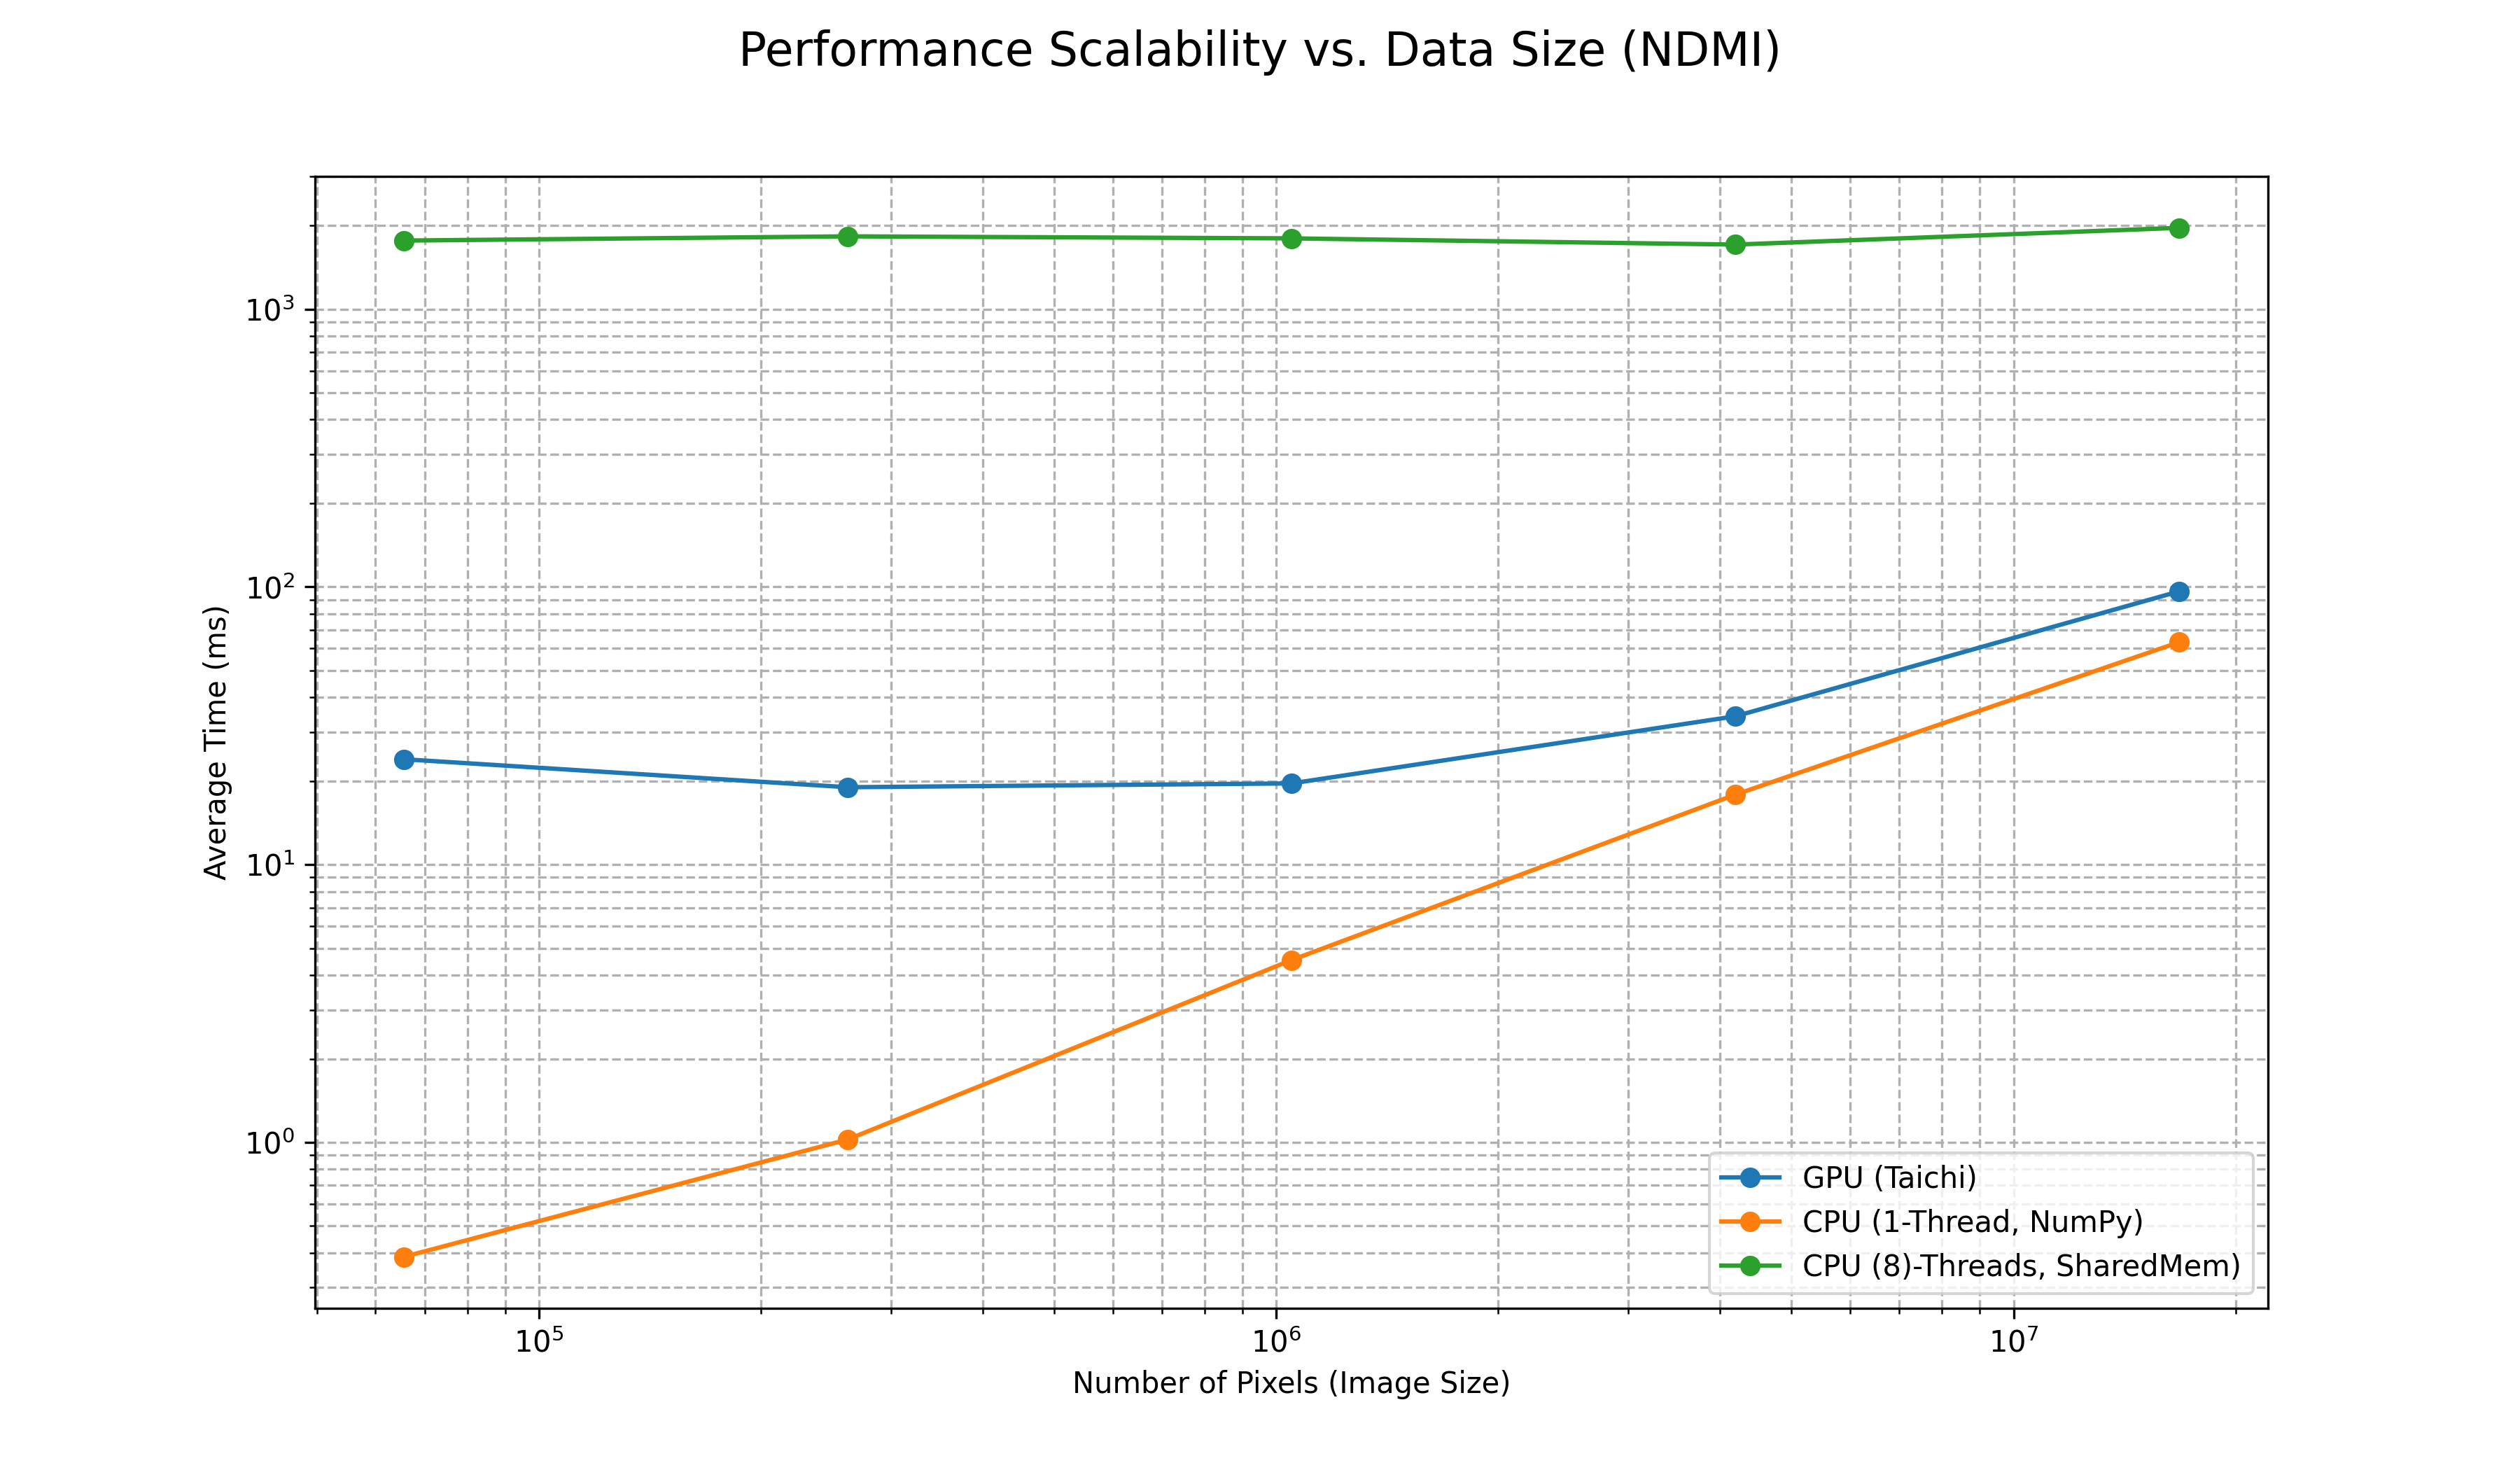
\includegraphics[width=\textwidth]{charts/04_size_scalability_ndmi.png}
    \caption{Skalowalność wydajności w zależności od rozmiaru danych (NDMI).}
    \label{fig:size_scaling_ndmi}
\end{figure}

\begin{figure}[H]
    \centering
    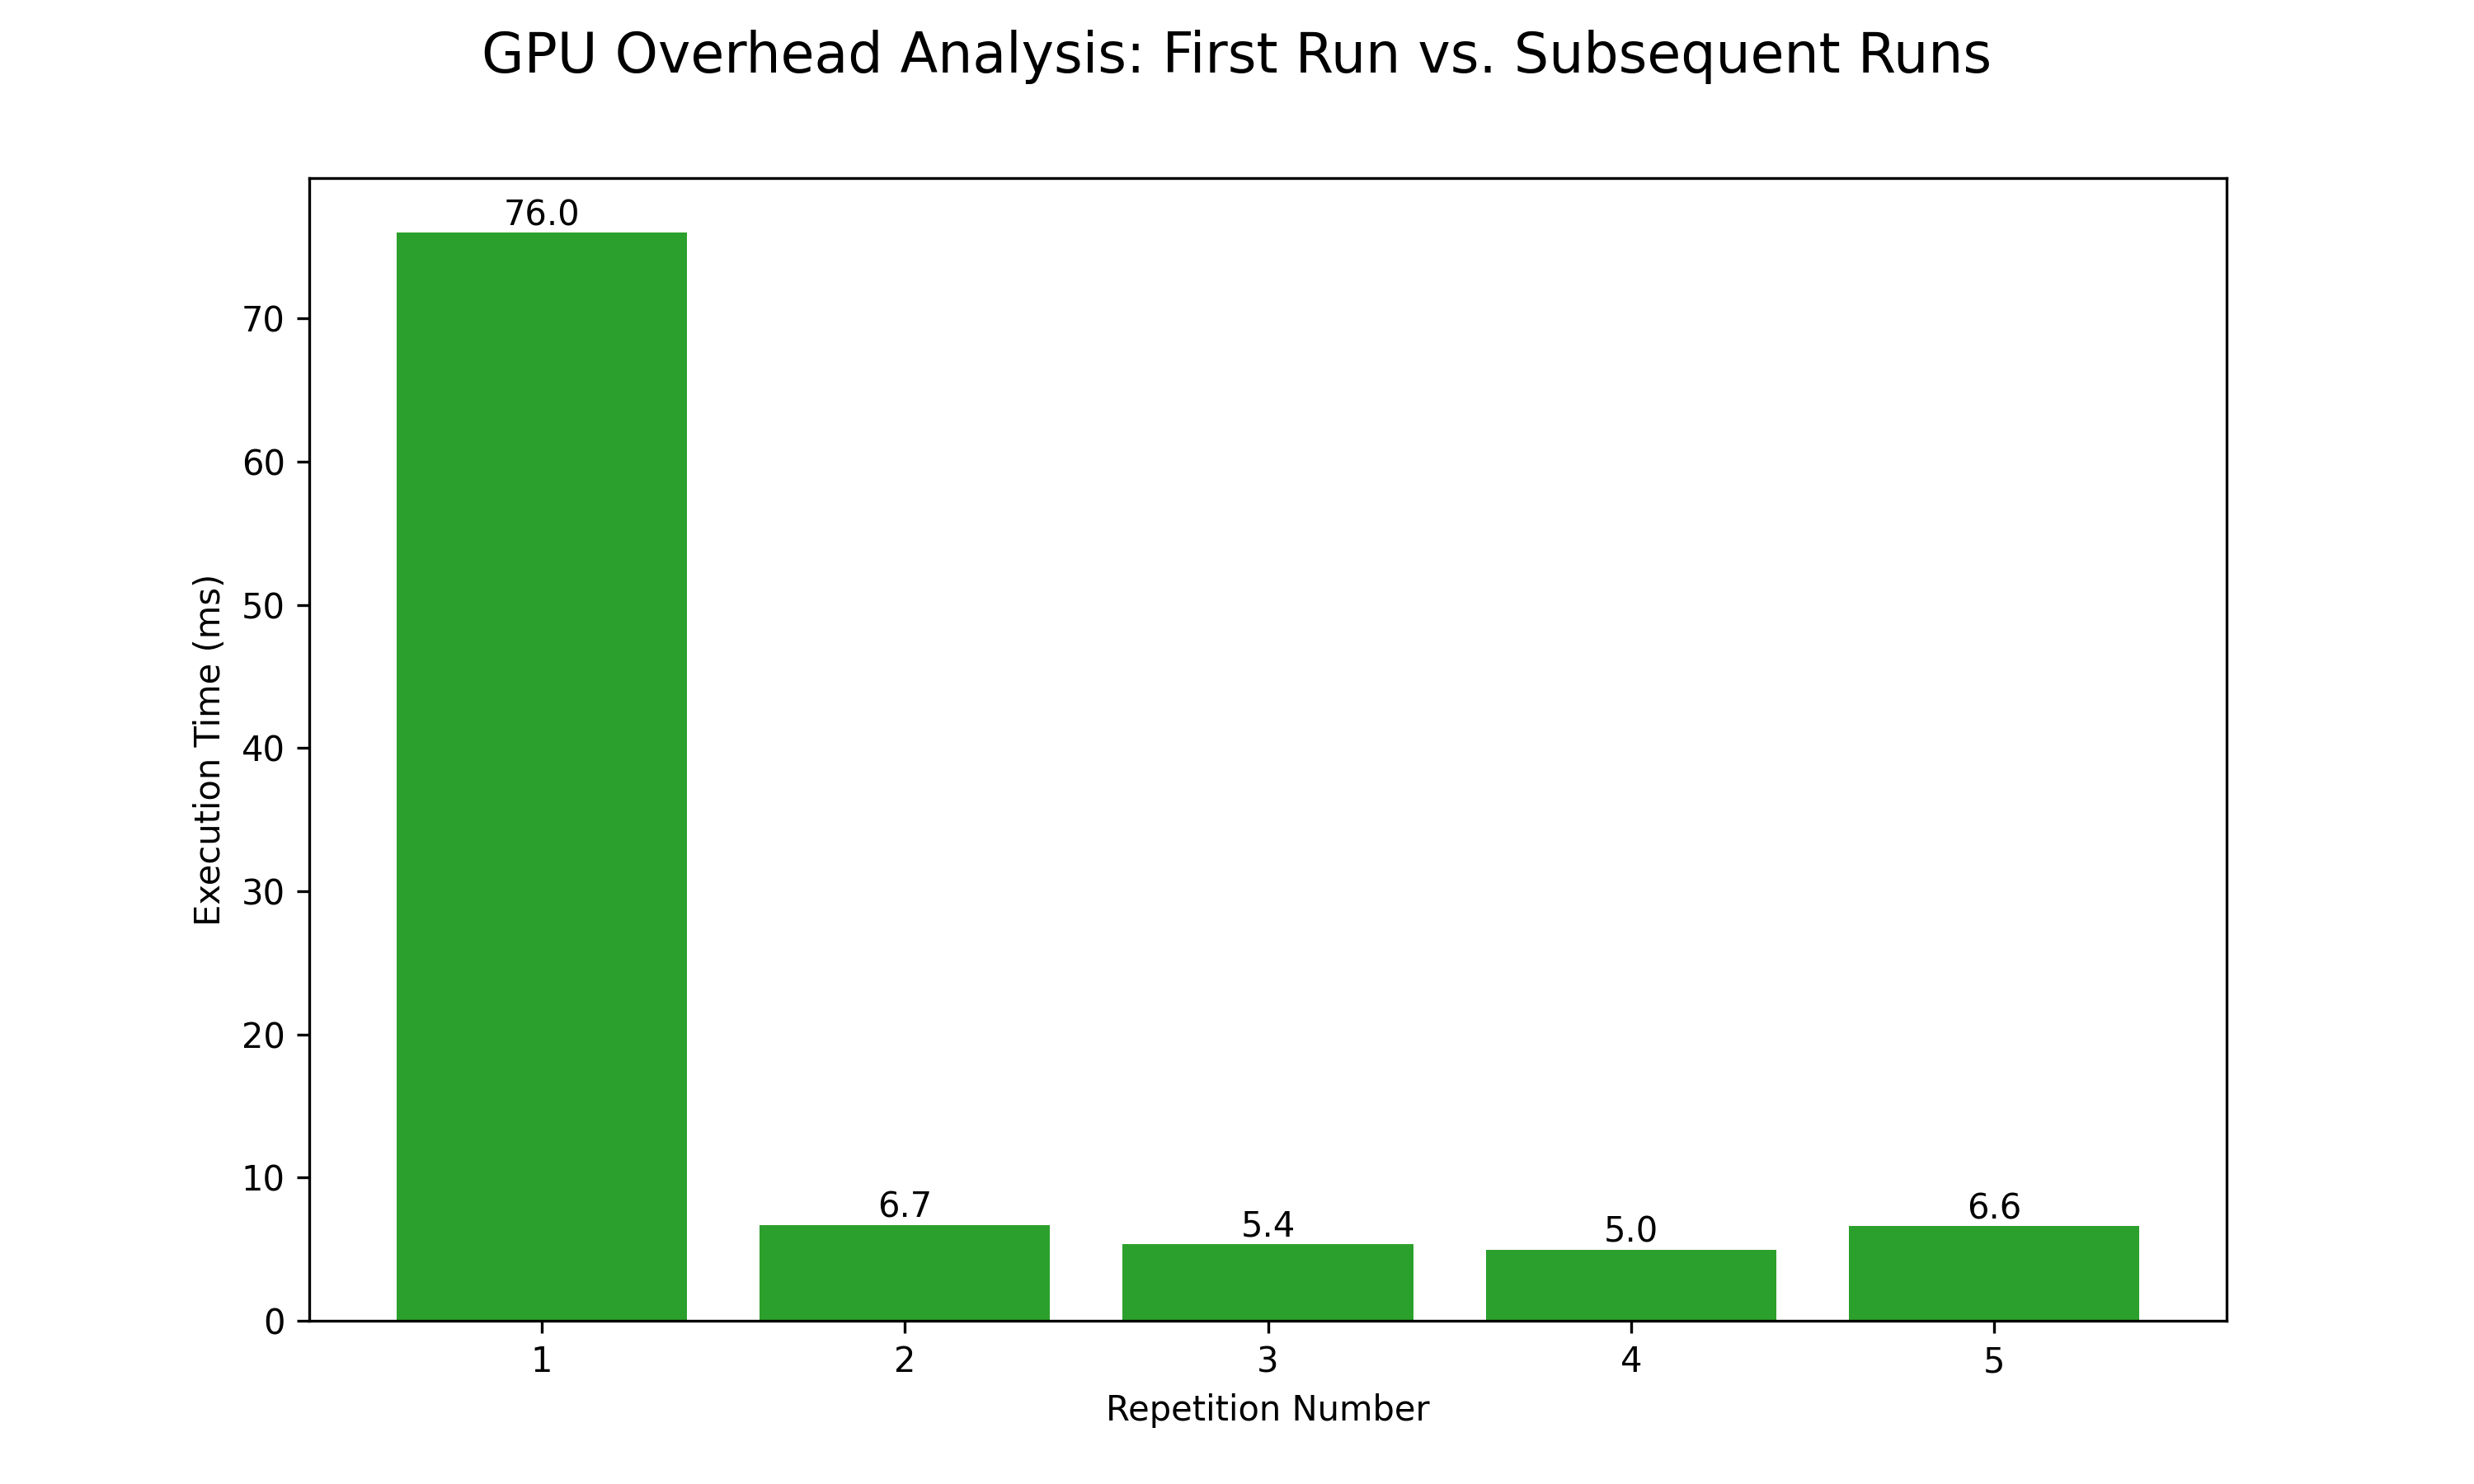
\includegraphics[width=0.8\textwidth]{charts/05_gpu_overhead.png}
    \caption{Analiza narzutu inicjalizacyjnego (warm-up) dla GPU.}
    \label{fig:gpu_overhead}
\end{figure}

\begin{figure}[H]
    \centering
    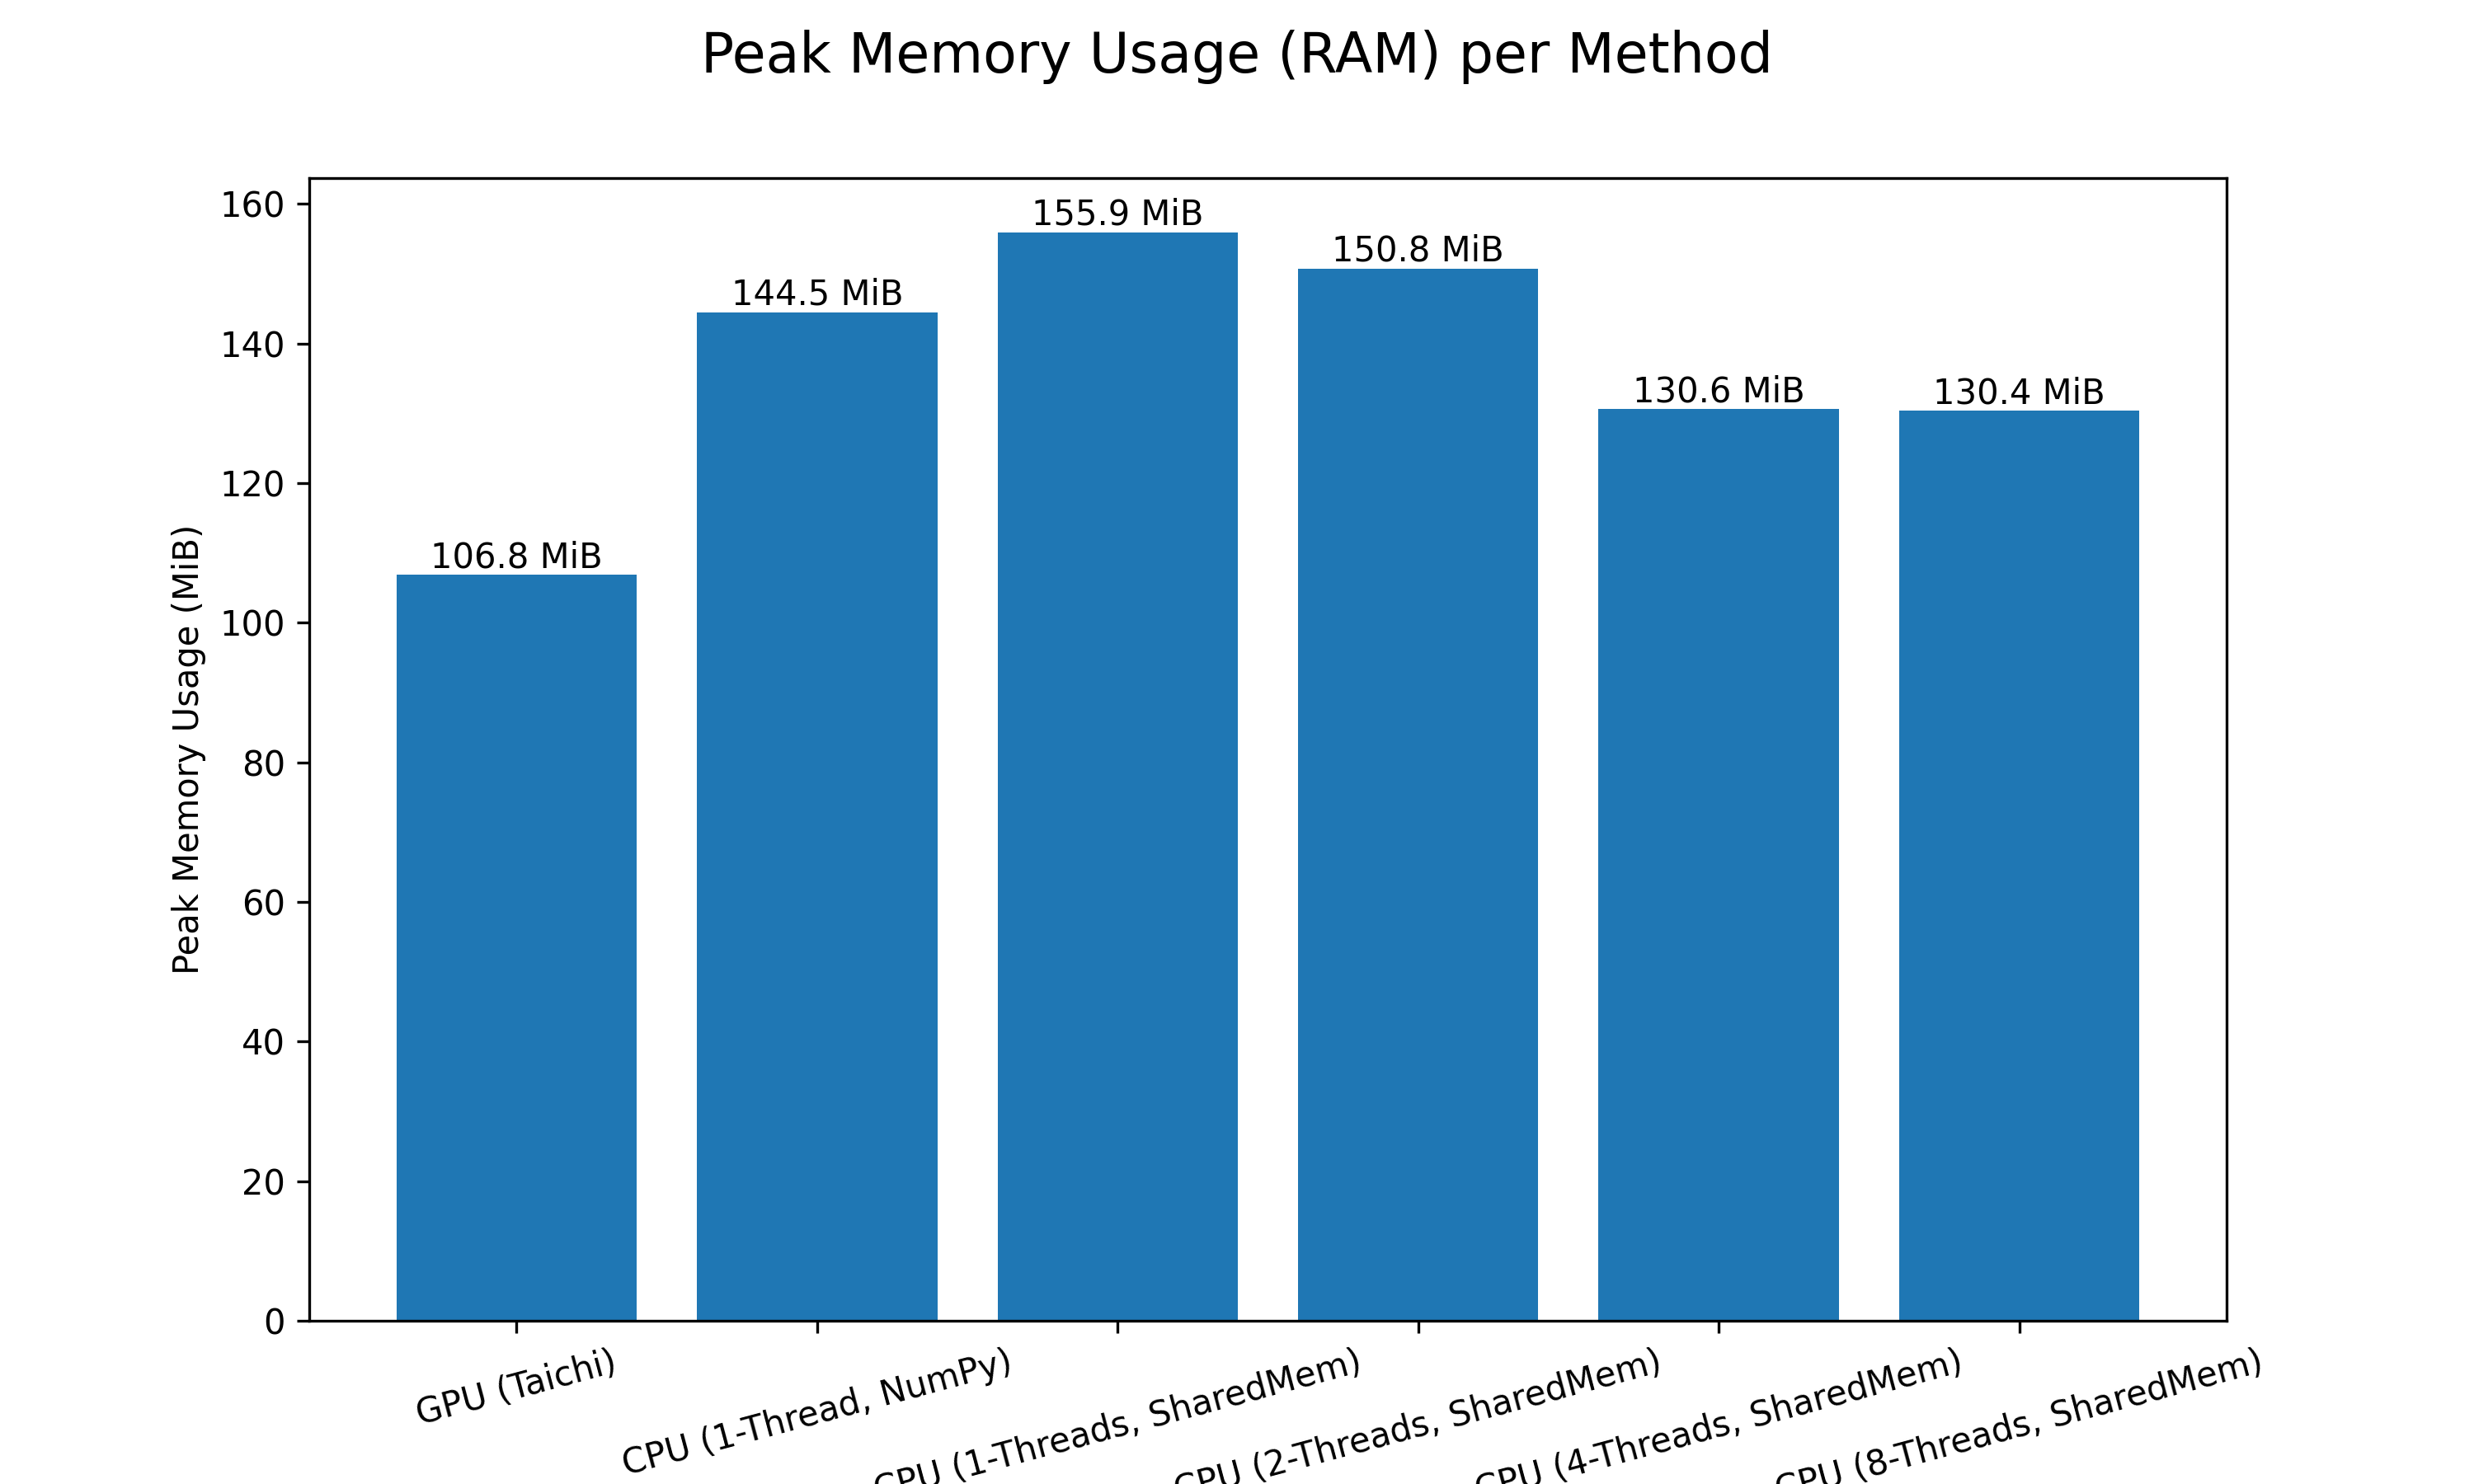
\includegraphics[width=0.8\textwidth]{charts/06_memory_usage.png}
    \caption{Szczytowe zużycie pamięci RAM przez proces główny.}
    \label{fig:memory}
\end{figure}

\newpage

\section{Interpretacja i wnioski}
Przeprowadzone testy porpzez wykresy, pozwalają na sformułowanie kluczowych wniosków dotyczących wydajności i zasadności stosowania różnych technik przetwarzania równoległego dla naszego problemu.

\subsection{Wniosek 1: Zoptymalizowany CPU jest najszybszy dla małych i średnich zadań}
Jak widać na Rysunku \ref{fig:overview}, dla standardowego zadania (obraz 1024x1024), wysoce zoptymalizowana, jednowątkowa implementacja oparta na NumPy jest ewidentnie najszybsza. Jest tak bo obliczenia są na tyle proste, że koszt narzutu związany z przeniesieniem danych do GPU lub zarządzaniem pulą procesów na CPU jest znacznie większy niż zysk z samego zrównoleglenia.

\subsection{Wniosek 2: Przetwarzanie równoległe na CPU ponosi znaczący koszt narzutu}
Rysunek \ref{fig:cpu_scaling} doskonale ilustruje problem narzutu w~`multiprocessing`. Czas wykonania dla jednego procesu w puli jest drastycznie wyższy niż dla wersji jednowątkowej bez puli. Wynika to z konieczności tworzenia nowych procesów, konfiguracji pamięci dzielonej i komunikacji międzyprocesowej. Mimo że implementacja poprawnie skaluje się wraz z dodawaniem kolejnych procesów (czas maleje), nigdy nie jest w stanie zniwelować początkowego narzutu i pokonać wydajności czystego NumPy dla tego zadania.

\subsection{Wniosek 3: GPU staje się opłacalne dopiero przy odpowiednio dużym rozmiarze problemu}
Analiza skalowalności w zależności od rozmiaru danych (Rysunki \ref{fig:size_scaling_ndvi} i \ref{fig:size_scaling_ndmi}) jest najważniejszym wynikiem projektu. Obserwujemy, że linia wydajności GPU - niebieska ma mniejsze nachylenie niż linia CPU - pomareńczowa, co oznacza, że lepiej radzi sobie z rosnącym obciążeniem. Widzimy wyraźny \textbf{punkt przełamania (break-even point)} w okolicach \(2 \cdot 10^6\) pikseli. Poniżej tego progu, zoptymalizowany CPU jest szybszy. Powyżej tego progu, zysk z masowego zrównoleglenia na GPU zaczyna przewyższać stały koszt transferu danych, czyniąc GPU metodą wydajniejszą dla bardzo dużych zbiorów danych.

\subsection{Wniosek 4: Analiza narzutu GPU i zużycia pamięci}
Rysunek \ref{fig:gpu_overhead} potwierdza istnienie kosztu "rozgrzewki" GPU. Pierwsze uruchomienie jest znacznie wolniejsze z powodu kompilacji JIT. Rysunek \ref{fig:memory} pokazuje z kolei kompromisy w zarządzaniu pamięcią. Metoda GPU odciąża systemową pamięć RAM, gdyz przenosi dane do VRAM.

\subsection{Wniosek ogólny: Wybór metody zależy od kontekstu}
Nie istnieje jedna, uniwersalnie najlepsza metoda. Wybór optymalnej strategii zależy od konkretnego przypadku użycia i konkretnych parametró wejściowych:
\begin{itemize}
    \item \textbf{Interaktywna analiza małych obszarów:} Wyraźnie widać, że najlepszym wyborem jest zoptymalizowany, jednowątkowy CPU (NumPy) ze względu na minimalny czas latencji.
    \item \textbf{Przetwarzanie wsadowe bardzo dużych obrazów:} Dla zadań przekraczających "punkt przełamania", GPU oferuje najwyższą przepustowość i jest metodą preferowaną.
    \item \textbf{Efektywność energetyczna:} Dla zadań, gdzie CPU jest szybsze, jest ono również znacznie bardziej efektywne energetycznie.
\end{itemize}
Wyniki te prezentują, jak kluczowe jest zrozumienie charakterystyki problemu (złożoność obliczeniowa vs. obciążenie I/O) oraz narzutów platformy przy projektowaniu systemów o wysokiej wydajności.

\section{Jak uruchomić program}
Aby uruchomić aplikację, należy postępować zgodnie z poniższymi krokami:

\begin{enumerate}
    \item Sklonować repozytorium projektu i przejść do jego głównego katalogu.
    \item Utworzyć i aktywować środowisko wirtualne z użyciem Pythona 3.11:
    \begin{lstlisting}[language=bash]
python3.11 -m venv venv
source venv/bin/activate
    \end{lstlisting}
    (Na Windows zamiast \texttt{source venv/bin/activate} należy użyć \texttt{venv\textbackslash Scripts\textbackslash activate}.)
    \item Zainstalować wszystkie wymagane biblioteki za pomocą menedżera pakietów pip:
    \begin{lstlisting}[language=bash]
pip install -r requirements.txt
    \end{lstlisting}
    
    \item Stworzyć plik \texttt{.env} w głównym katalogu projektu. Plik ten będzie zawierał \textbf{jedynie} sól kryptograficzną, która jest niezbędna do odszyfrowania danych logowania. Dla celów testowych i odtworzenia wyników, należy użyć poniższej wartości:
    \begin{lstlisting}
SENTINEL_SALT="385d0b98fb81618a8d5165a2c25300e26217c22661ca9ada7cde877075184219"
    \end{lstlisting}
    
    \item Przygotować własne dane uwierzytelniające (Client ID oraz Client Secret) do API Sentinel Hub. Instrukcje, jak je uzyskać, znajdują się w oficjalnej dokumentacji: \url{https://docs.sentinel-hub.com/api/latest/api/overview/authentication/}.
    
    \item Przy pierwszym uruchomieniu, aplikacja poprosi o podanie uzyskanych danych oraz o hasło, które posłuży do ich zaszyfrowania i bezpiecznego przechowania w pliku \texttt{sentinel\_config.enc}. Dla celów ewaluacji projektu, w repozytorium znajduje się już gotowy plik \texttt{sentinel\_config.enc}, do którego hasło zostanie udostępnione osobno.
    
    \item Uruchomić główną aplikację za pomocą polecenia z \textbf{głównego katalogu projektu}:
    \begin{lstlisting}[language=bash]
python -m src.main
    \end{lstlisting}
    \textit{Uwaga: Użycie flagi \texttt{-m} jest kluczowe, ponieważ zapewnia, że Python poprawnie rozpoznaje strukturę pakietów w folderze \texttt{src}.}
\end{enumerate}

\subsection{Uruchamianie skryptów testowych (opcjonalne)}
Aby przeprowadzić testy wydajności i pamięci, należy najpierw wygenerować dane testowe, a następnie uruchomić skrypt profilujący. Oba skrypty należy uruchamiać z \textbf{głównego katalogu projektu}.

\begin{enumerate}[label*=\arabic*.]
    \item Generowanie danych testowych o różnej skali:
    \begin{lstlisting}[language=bash]
python -m src.scripts.generate_scaled_data
    \end{lstlisting}
    \item Uruchomienie testów zużycia pamięci (wymaga \texttt{memory-profiler}):
    \begin{lstlisting}[language=bash]
python -m memory_profiler src.scripts.run_memory_tests
    \end{lstlisting}
\end{enumerate}


\printbibliography[heading=bibintoc]

\end{document}